\documentclass[12pt,a4paper]{article}

%% Package using
\usepackage[utf8]{inputenc}
\usepackage{xeCJK}          % 使用中文
\usepackage{graphicx}       % 插入圖片
\usepackage{indentfirst}    % 首段空格
\usepackage{listings}       % code block
\usepackage{xcolor}         % set color
\usepackage{amsmath}        % align

%% Document Style
\linespread{1.5}    % 行距    
\setCJKmainfont{NotoSansTC-Light.otf}[
Path=./Font/,
BoldFont=NotoSansTC-Regular.otf]     % 中文字型_黑體
\renewcommand{\familydefault}{\sfdefault}   % 英文字型_sans font
\renewcommand\contentsname{目錄}            % TOC標題 : Content -> 目錄
\graphicspath{{./Pic/}}                     % 圖片路徑
\setlength{\parindent}{2em}                 % 首段空兩格


% Code block style
\definecolor{gray}{rgb}{0.5,0.5,0.5}
\definecolor{backColor}{HTML}{f7f6f2}
\definecolor{darkgreen}{HTML}{7f9353}
\definecolor{darkblue}{HTML}{629aaa}
\definecolor{darkred}{HTML}{d38696}

\lstset{
  inputpath=../,
  language=Matlab,
  basicstyle={\linespread{1.0}\ttfamily\small},
  backgroundcolor=\color{backColor},
  keywordstyle=\color{darkblue},
  identifierstyle=\color{darkred},
  commentstyle=\color{gray},
  stringstyle=\color{darkgreen},
  showstringspaces=false,
  keepspaces=true,
  columns=flexible,
  breaklines=true,
  breakatwhitespace=true,
  tabsize=4,
%   numbers=left,
%   stepnumber=1
}


%% Document Content
\begin{document}

% Title page
\begin{center}
    
    \vspace*{5cm}
    \textbf{\huge Orientation Homework Report}\\   % 粗體+加大
    
    \vspace{1cm}
    {\large 10-bar truss optimization}
    
    \vfill
    {\Large 徐若瑄}
    
    \vspace{1cm}
    {\Large \today}

\end{center}
\newpage

% %----------------Next Page--------------

% \tableofcontents

% \newpage
% %----------------Next Page--------------

% Section 1
\section{問題描述}

    十桿衍架(10-bar truss)由十個長桿件組成並且有6個端點,其中第5、6號端點為固定端,桿件的配置如圖\ref{10-bar truss}所示。
    
    \begin{figure}[h]
        \centering
        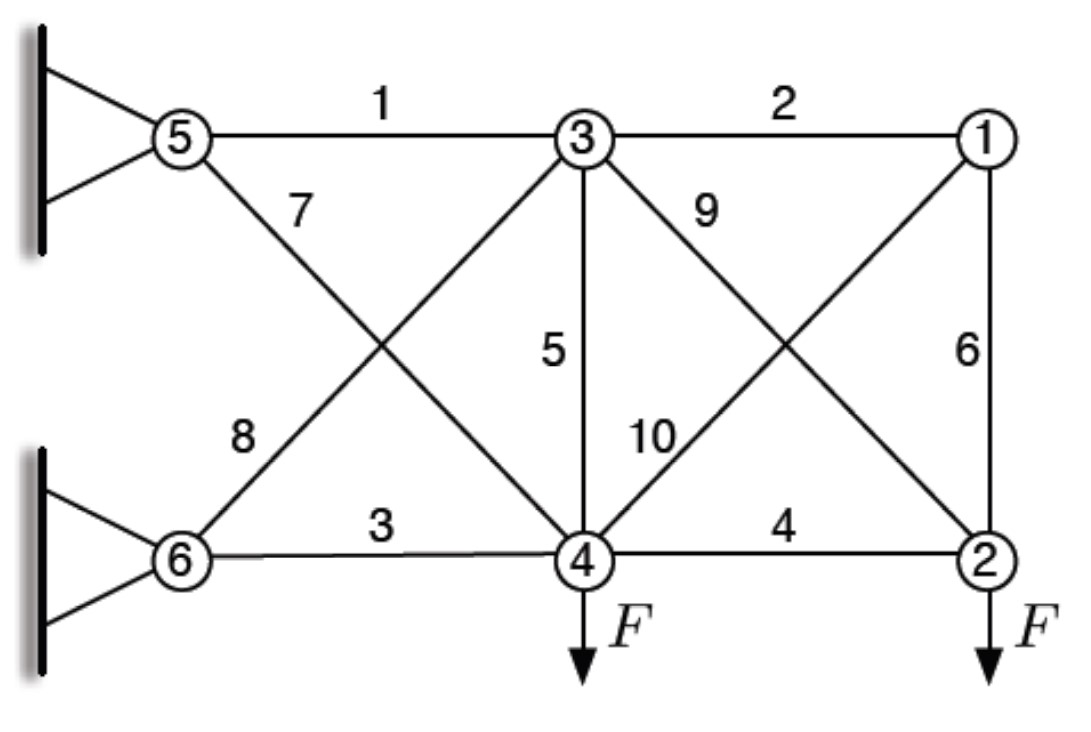
\includegraphics[width=8cm]{10_bar_truss}
        \caption{10-bar truss}
        \label{10-bar truss}
    \end{figure}
    
    所有桿件的截面皆為圓形,桿件1到桿件6的截面半徑同為$r1$且長度為$9.14\  m$;桿件7到桿件8的截面半徑同為$r2$。
    桿件所使用的材料為剛,相關的材料性質有:
    
    \begin{enumerate}
        \item 密度 $\rho = 7860\ kg/m^3$
        \item 楊氏模數(Young's Modulus) $E = 200\ GPa$
        \item 降伏係數(Yield stress) $\sigma_y = 250\ MPa$
    \end{enumerate}
    
    端點4及端點5有一向下的外力$F = 1.0x10^-7\ N$,
    在所有桿件的應力不超過降伏應力且端點2的位移小於$0.02\ m$的條件下,
    求桿件截面半徑$r1$與$r2$的值,使得十桿衍架整體重量為最輕。
    
\newpage
%----------------Next Page--------------

% Section 2
\section{計算方法}
    
    計算十桿衍架最小重量主要使用兩個方法,首先利用有限元素法(Finite element method)計算出所有桿件的應力值、各個端點的位移量,接著進行最佳化即可得到最佳值與最佳解。
    
    以下所有計算過程皆使用Matlab程式輔助計算。
    
    \subsection{有限元素分析}
        
        有限元素分析的關鍵步驟如下:
        \begin{enumerate}
            \item 建立元素表(Element Table):
                  元素表內包含各桿件的長度、截面積、角度等
            \item 建立剛性矩陣(Stiffness Matrix):
                  利用元素表計算出剛性矩陣$K$,表示出6個端點的12個自由度上下位移與受力之間的關係
            \item 計算各個節點的位移:
                  透過$F=KQ$的關係式求出各點在x,y兩方向的位移量
            \item 計算各桿件的應力:
                  透過$\sigma=E\varepsilon$的關係式求出各桿件的應力
            \item 計算反作用力:
                  同樣使用$F=KQ$的關係式求出固定端點5、6的反作用力
            \item 最佳化:
                  將問題條件轉換為數學式,最佳化後得到最佳值與最佳解
        \end{enumerate}
        
        \newpage
%----------------Next Page--------------

        \subsubsection{建立端點與桿件參數}
        
            為了快速建立元素表,首先將桿件長度轉換為各端點的座標位置(以端點6為原點)並存於\texttt{nodeTable}
            \lstinputlisting[firstline=10,lastline=16]{finiteElementMethod.m}
            
            接著設定桿件1到桿件10對應到的左右兩截點編號。
            利用\texttt{nodeInfo}紀錄各端點連接的桿件編號,
            再將桿件兩端點的編號存於\texttt{elementToNode}
            \lstinputlisting[firstline=18,lastline=29]{finiteElementMethod.m}
            

        \subsubsection{建立元素表}
            
            元素表\texttt{elementTable} 為10x4的矩陣,
            每一欄依序紀錄各桿件的
            \begin{enumerate}
                \item 長度 
                        \begin{math}
                            L=\sqrt{\left(x_{nodej}-x_{nodei}\right)^2+
                                    \left(y_{nodej}-y_{nodei}\right)^2}
                        \end{math}
                \item 截面積 $A=\pi\times r^2$
                \item 餘弦 $cos\theta_e=\displaystyle\frac{\left(x_{nodej}-x_{nodei}\right)}{L}$
                \item 正弦 $sin\theta_e=\displaystyle\frac{\left(y_{nodej}-y_{nodei}\right)}{L}$
            \end{enumerate}

            以\texttt{elementToNode}搭配\texttt{nodeTable}取得各端點的$x,y$座標值,
            根據上方提供的公式計算各項數值
            \lstinputlisting[firstline=41,lastline=67]{finiteElementMethod.m}

        \newpage
        \subsubsection{剛性矩陣}

            剛性矩陣(Stiffness Matrix)為表示各端點的位移與受力關係的矩陣,在數學式中以$K$表示。
            各桿件皆存在左右兩端點,因此其剛性矩陣大小為4x4,表示出4個自由度(Degree of freedom,DOF)位移與受力的關係,
            其公式如下:
            \begin{displaymath}
                k^e = \frac{EA_e}{L_e}\left[
                    \begin{array}{cccc}
                        c^2 & cs & -c^2 & -cs\\
                        cs & s^2 & -cs & -s^2\\
                        -c^2 & -cs & c^2 & cs\\
                        -cs & -s^2 & cs & s^2
                    \end{array}\right]
            \end{displaymath}

            十桿衍架有6個端點且每個端點皆有2個DOF,
            端點1的$x$方向DOF以1表示;端點1的$y$方向DOF以2表示,依序到第12個DOF表示端點6的$y$方向。
            以桿件2及桿件6的剛性矩陣為範例,其矩陣各行及各列所表示的DOF依序為
            左端點的$x$方向、左端點的$y$方向、右端點的$x$方向及右端點的$y$方向:
            \begin{figure}[h]
                \centering
                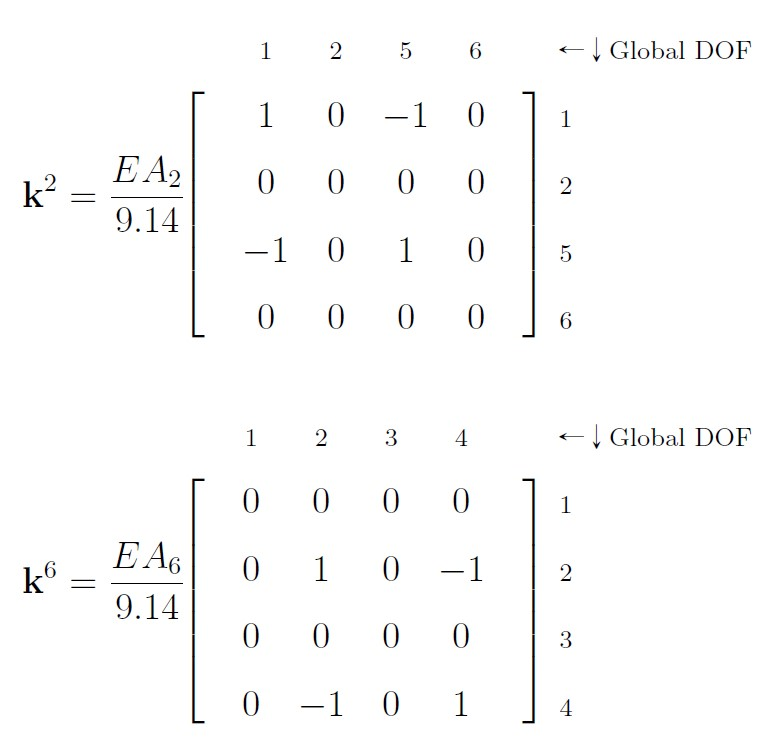
\includegraphics[width=8cm]{Stiffness_matrix_GlobalDOF}
            \end{figure}

            將所有桿件的剛性矩陣加總即可得到十桿衍架整體的剛性矩陣:
            \begin{displaymath}
                \mathbf{K} \leftarrow \sum_{e=1}^{10} \mathbf{k}^e
            \end{displaymath}

            % \newpage
            \texttt{elementTable}中提供計算剛性矩陣所需的$L_e,A_e,cos,sin$,\\
            以\texttt{elementToNode}取得桿件的4個DOF值,
            並依序將計算的結果加總至\texttt{stiffnessMatrix}中對應的DOF欄位
            \lstinputlisting[firstline=72,lastline=93]{finiteElementMethod.m}
        
        \newpage
        \subsubsection{節點位移}

            使用前一步驟所得到的剛性矩陣及已知的受力,即可求得各節點的位移:
            \begin{displaymath}
                \mathbf{F} = \mathbf{K}\mathbf{Q}
            \end{displaymath}
            由於端點5、端點6為固定點,因此$x,y$方向位移皆為0:
            \begin{displaymath}
                Q_9=Q_{10}=Q_{11}=Q_{12}=0
            \end{displaymath}
            也因此可將剛性矩陣簡化為8x8的矩陣:
            \begin{displaymath}
                \mathbf{F}_{8\times1} = \mathbf{K}_{8\times8}\times\mathbf{Q}_{8\times1}
            \end{displaymath}
            等式兩邊同乘$K^{-1}$:
            \begin{displaymath}
                \mathbf{K}^{-1}\mathbf{F} = \mathbf{Q}
            \end{displaymath}

            將原為12x12的\texttt{stiffnessMatrix}複製到
            \texttt{stiffness\_disp}並轉換為8x8的矩陣,
            利用上述公式計算DOF1~DOF8的位移量
            \lstinputlisting[firstline=95,lastline=109]{finiteElementMethod.m}

        \subsubsection{桿件應力}

            楊式係數(Young's Modulus)的定義為應力與應變的比值:
            \begin{displaymath}
                E = \frac{\sigma}{\varepsilon}
            \end{displaymath}
            其中應變$\varepsilon$可由上一步驟所得到的位移轉換而成:
            \begin{displaymath}
                \varepsilon = \frac{\delta}{L} = \frac{1}{L}\left[
                \begin{array}{cccc}
                    -c & -s & c & s
                \end{array}
                \right]\times\mathbf{Q}
            \end{displaymath}
            因此各桿件所受到的應力大小為:
            \begin{displaymath}
                \sigma_e = \frac{E_e}{L_e}\left[
                    \begin{array}{cccc}
                        -c & -s & c & s
                    \end{array}
                    \right]\times\mathbf{Q}
            \end{displaymath}

            同樣使用\texttt{elementTable}取得$L_e,cos,sin$的值,並搭配\\
            \texttt{elementToNode}將各桿件的相關DOF位移存於\texttt{disp\_element},
            最後利用上述公式求得桿件應力
            \lstinputlisting[firstline=112,lastline=136]{finiteElementMethod.m}
            
        \subsubsection{反作用力}

            由於端點5、端點6為固定點,因此在此會有反作用力的產生。
            與2.1.4中提到的計算方式相同,因為只計算DOF9~DOF12的作用力,
            因此將剛性矩陣調整為4x12的大小:
            \begin{displaymath}
                \mathbf{F}_{4\times1} = \mathbf{K}_{4\times12}\times\mathbf{Q}_{12\times1}
            \end{displaymath}

            將原為12x12的\texttt{stiffnessMatrix}複製到
            \texttt{stiffness\_reac}並轉換為4x12的矩陣,
            利用上述公式計算反作用力數值
            \lstinputlisting[firstline=138,lastline=148]{finiteElementMethod.m}
    
    \newpage
    \subsection{最佳化}

        最佳化數學表示式為:
        \begin{align*}
            \min_{r1,r2}\quad & f\left(r1,r2\right) = \sum_{i=1}^6m_i(r_1) + \sum_{i=7}^{10}m_i(r_2) \\
            \mbox{subject to}\quad & |\sigma_i| \leq \sigma_y \\
                               & \Delta s_2 \leq 0.02
        \end{align*}
        
        於Matlab中使用\texttt{fmincon}進行最佳化運算,
        將計算最小值運算式存於\textbf{\texttt{obj.m}}
        \lstinputlisting[firstline=1,lastline=18]{obj.m}
        限制條件則於\textbf{\texttt{nonlcon.m}}中進行設定,並於此副函式執行\\
        \textbf{\texttt{finiteElementMethod.m}}的有限元素分析以取得位移及應力數值
        \lstinputlisting[firstline=1,lastline=22]{nonlcon.m}
        \lstinputlisting[firstline=1,lastline=1]{finiteElementMethod.m}
        主函式\textbf{\texttt{Hw.m}}則用來執行\texttt{fmincon}計算最佳值、最佳解;
        同時於主函式中存取常數(楊式係數、密度、長度、降伏應力)的值並設為廣域變數,
        日後修改參數及程式維護較便利,及函式間的取值也較不易有錯誤產生
        \lstinputlisting[firstline=19,lastline=30]{Hw.m}
        \lstinputlisting[firstline=5,lastline=10]{Hw.m}


\newpage
%----------------Next Page--------------

% Section 3
\section{結論}

\end{document}
